\documentclass[11pt, oneside]{article}
\usepackage[utf8]{inputenc}                        % utf8
\usepackage[T1]{fontenc}                           % fix font encoding
\usepackage[english]{babel}                        % language
\usepackage{titling, geometry, hyperref, fancyhdr, algorithm, physics}
\usepackage{amsmath, amssymb, amsthm, mathtools}   % mathematical packages
\usepackage{graphicx, subcaption, wrapfig}         % images
\usepackage{fvextra, textcomp, CJKutf8}            % misc. text formatting
\usepackage[autostyle, english=american]{csquotes} % quotes
\usepackage[shortlabels]{enumitem}                 % lists
\usepackage{tikz, pgfplots, tikz-network}          % plots and graphs
\usepackage[noend]{algpseudocode}                  % algorithm psuedocode
\usepackage[cache=true]{minted}                    % source code
\usepackage[style=ieee]{biblatex}                  % bibliography
\geometry{a4paper}

\pgfplotsset{compat=1.17}                          % version of pgfplots

\hypersetup{
  colorlinks=true,
  urlcolor=cyan,
  linkcolor=black
}

\setminted[]{
  linenos=false,
  breaklines=true,
  encoding=utf8,
  fontsize=\normalsize,
  frame=lines,
  framesep=2mm
}

% https://tex.stackexchange.com/questions/343494/minted-red-box-around-greek-characters
\makeatletter
\AtBeginEnvironment{minted}{\dontdofcolorbox}
\def\dontdofcolorbox{\renewcommand\fcolorbox[4][]{##4}}
\makeatother

\newcommand{\emphasis}[1]{\textbf{\textit{#1}}}
\graphicspath{{./images/}}
\addbibresource{ref.bib}

\theoremstyle{plain}
\newtheorem{theorem}{Theorem}[section]
\newtheorem{corollary}{Corollary}[theorem]
\newtheorem{lemma}[theorem]{Lemma}

\theoremstyle{definition}
\newtheorem{definition}{Definition}[section]
\renewcommand\qedsymbol{$\square$}

\DeclareMathOperator{\FFT}{FFT}

\title{Fast Fourier Transform and 2D Convolutions}
\author{Stephen Huan}
\date{October 16, 2020}

\begin{document}
\maketitle
% \tableofcontents

\section{Introduction}

The Fast Fourier Transform (FFT) is a common technique for signal processing
and has many engineering applications. It also has a fairly deep mathematical
basis, but we will ignore both those angles in favor of accessibility.
Instead, we will approach the FFT from the most intuitive angle,
\emphasis{polynomial multiplication}.
First, we represent polynomials by a list of coefficients,
where the number at index 0 represents the coefficient of \( x^0 \),
the number at index 1 represents the coefficient of \( x^1 \), and so on.
For example, the polynomial \( 3 + 2x + 4x^2 \) becomes [3, 2, 4].

The multiplication of two polynomials \( f \) and \( g \) is then simply
each term of \( f \) multiplied with each term of \( g \) and then added up.
We can also assume that \( f \) and \( g \) are the same length \( N \),
where the polynomial of lesser degree is padded with zeros.
If we say the product is \( p \), we can give an formula
for an index in \( p \) in the following way:
\[ p[n] = (f * g)[n] = \sum^n_{i = 0} f[i]g[n - i] \]
\( p[n] \) is the coefficient of \( x^n \) in the product, and it is formed
by adding up all the possible ways to get to \( x^n \), i.e. \( f[0] x^0 \)
times \( g[n] x^n \), \( f[1] x^1 \) times \( g[n - 1] x^{n - 1} \), etc.
Intuitively, this \enquote{flips} \( g \), and then the resulting product
is computed by \enquote{sliding} \( g \) over \( f \) and then computing
the dot product between the two lists, or a weighted average.

Sticking with the example from before, we have the polynomial [3, 2, 4]
and the polynomial \( 1 + 3x + 2x^2 \) = [1, 3, 2]. To compute their
product, we first flip the second list to get [2, 3, 1]. We then slide [2, 3, 1]
over [3, 2, 4], imagining there are zeros such that the parts of [2, 3, 1]
that don't overlap with [3, 2, 4] aren't counted.
For the first value, 1 overlaps with 3 so we get 3. 
Then, [3, 1] overlaps with [3, 2] so we get \( 3 \cdot 3 + 1 \cdot 2 = 11 \).
[2, 3, 1] overlaps with [3, 2, 4] \( = 16 \), [2, 3] overlaps [2, 4] \( = 16 \),
and finally [2] overlaps with [4] to give 8.
Our final answer is then [3, 11, 16, 16, 8] = \( 3 + 11x + 16x^2 + 16x^3 + 8x^4
= (3 + 2x + 4x^2)(1 + 3x + 2x^2) \).

What if we computed \( g * f \)? It should be the same since
polynomial multiplication should be commutative, but we can prove it.
\begin{theorem}
    \( f * g = g * f \), i.e. polynomial multiplication is commutative.
\end{theorem}
\begin{proof}
    We have \( (f * g)(n) = \sum^n_{i = 0} f[i]g[n - i] \) by definition.
Perform the variable substitution \( k = n - i \), so \( i = n - k \).
Summing from \( \sum^n_{i = 0} \) will sum from \( k = n \) to \( k = 0 \)
in descending order, so \( \sum^n_{i = 0} = \sum^n_{k = 0} \)
(from the commutativity of addition).
\begin{align*}
    (f * g)[n] &= \sum^n_{i = 0} f[i]g[n - i] && \text{Definition} \\
               &= \sum^n_{k = 0} f[n - k]g[k] && \text{Substitution} \\
               &= (g * f)
\end{align*}
\end{proof}

This operation is known as a \emphasis{convolution}, which is equivalent to
polynomial multiplication in the discrete case and is denoted \( f * g \).
Its relevance to image processing will be expounded on later
(for now, this puts the \enquote{convolutional}
in \enquote{Convolutional Neural Networks}).
Today's lecture is about the \emphasis{Fast Fourier Transform}, an efficient
algorithm to perform convolutions.

\section{Algorithms}
A naive approach to the convolution of two lists of length \( N, M \) will have
runtime \( O(NM) \) using the standard polynomial multiplication algorithm
(each term of the first list multiplied with each term of the second list).
However, the length of the convolution will be \( N + M - 1 \).
The first list is a polynomial of degree \( N - 1 \),
the second of degree \( M - 1 \), so the resulting polynomial has degree 
\( (N - 1) + (M - 1) = N + M - 2 \). A polynomial of degree \( D \)
has \( D + 1 \) coefficients, so the length of the product is \( N + M - 1 \).
Thus, the lower bound for a convolution is linear,
so a better runtime than quadratic could exist. 

\subsection{FFT}
\subsubsection{Point-Value Representation}
The key observation is that we can represent polynomials in a different form
than a coefficient list. In particular, we can use a \emphasis{point-value}
representation, or a list of \( (x, y) \) pairs that give an input and the
corresponding output of a polynomial. We call the process of going from
a coefficient representation to a point-value representation
\emphasis{evaluation}, since we evaluate the polynomial at multiple points
to get the point-value representation. Likewise, we call the process of going
from a point-value representation to a coefficient representation
\emphasis{interpolation}, since we are finding a polynomial which \enquote{fits}
the data. Suppose we have a polynomial of degree \( n \). We then need
a certain number of points for evaluation and interpolation to be well-defined.
Evaluation is always well-defined, because we can always evaluate a polynomial
of any degree or coefficient representation. However, if we don't have
enough points, interpolation is not necessarily possible. For example, consider
the point-value representation \( [(0, 0), (1, 1)] \) and a degree of 2.
This could be the polynomial \( x^2 \) or \( 2x^2 - x \).
So for a polynomial of degree \( n \), we need at least \( n + 1 \)
distinct points (since each point gives another linear equation constraining
the \( n + 1 \) coefficients of the polynomial). 
We can in fact prove that if we have \( n + 1 \) points, that uniquely
determines a polynomial of degree \( n \).
\begin{theorem}
    A point-value representation with \( n \) distinct points uniquely
    determines a polynomial of degree \( n - 1 \).
\end{theorem}
\begin{proof}
We have a polynomial of the form
\( p(x) = a_0 + a_1 x + a_2 x^2 + \dots + a_{n - 1} x^{n - 1} \) and \( n \) points
of the form \( (x_i, y_i) \) such that \( p(x_i) = y_i \). 
Those constraints determine the following matrix equation:
\[
\begin{bmatrix}
  1 & x_0 & x^2_0 & \cdots & x^{n - 1}_0 \\
  1 & x_1 & x^2_1 & \cdots & x^{n - 1}_1 \\
  \vdots & \vdots & \vdots & \ddots & \vdots \\
  1 & x_{n - 1} & x^2_{n - 1} & \cdots & x^{n - 1}_{n - 1} \\
\end{bmatrix}
\begin{bmatrix}
  a_0 \\
  a_1 \\
  \vdots \\
  a_{n - 1}
\end{bmatrix}
=
\begin{bmatrix}
  y_0 \\
  y_1 \\
  \vdots \\
  y_{n - 1}
\end{bmatrix}
\]
The leftmost matrix is known as the \textit{Vandermonde matrix},
denoted \( V(x_0, x_1, \dots, x_{n - 1}) \) which has the determinant
(left as an exercise for the reader)
\[ \prod_{0 \leq j < i \leq n - 1} (x_i - x_j) \]
A matrix is invertible if and only if its determinant is nonzero,
so this matrix is invertible if each \( x_i \) is distinct. 
Thus, we can solve for the coefficients by multiplying by the inverse, so
\( \vec{a} = V^{-1} \vec{y} \), and this solution is unique since an invertible
matrix is a \textit{bijective} transformation between a vector space and itself.
\end{proof}

This proof directly gave an easy construction of the interpolating polynomial,
by \( V^{-1} \vec{y} \). Matrix inverses can be computed in \( O(n^3) \) as
an easy upper bound, but that can be improved with
\textit{Lagrange's interpolating formula} to yield a \( O(n^2) \) time
algorithm. I will not elaborate on Lagrange's formula in this lecture
but a good Wikipedia page is available
\href{https://en.wikipedia.org/wiki/Lagrange\_polynomial}{here}.

If we have a list of \( N \) coefficients, then the polynomial is of degree
\( N - 1 \) and thus we need \( N \) distinct points.
We first figure out how to evaluate polynomial at a single point,
and will repeat the process for all the points.
Suppose we have a polynomial of the form
\( p(x) = a_0 + a_1 x + a_2 x^2 + \dots + a_{n - 1} x^{n - 1} \). 
If we evaluate at a particular \( x_0 \), we compute each \( a_i {x_0}^i \) term
which would take \( O(N^2) \) time with repeated multiplication
and \( O(N \log N) \) time with fast exponentiation. 
But we can do better with \textit{Horner's rule}.
We notice that the degree in coefficient form is monotonically increasing,
so we can successively factor out a multiplication by \( x \).
\[ p(x) = a_0 + x (a_1 + x(a_2 + \dots + x(a_{n - 2} + x a_{n - 1}))) \] 
We do \( N \) multiplications and \( N \) additions, so the algorithm runs in
\( O(N) \). Evaluating a polynomial at \( N \) points then takes
\( O(N \cdot N) = O(N^2) \) time.

So we can do both evaluation and interpolation in \( O(n^2) \) and both are
well-defined if we have enough points. Why did we figure this out?
We can multiply two polynomials efficiently if we have the point-value
representations of each! Suppose we have polynomials \( f, g \) in
coefficient form. We also assume that the polynomials are evaluated at the
\textit{same} points, so we have \( [(x_0, f(x_0)), (x_1, f(x_1)), \dots ]\)
and \( [(x_0, g(x_0)), (x_1, g(x_1)), \dots ]\). \( f * g \) is then simply
\( [(x_0, f(x_0) g(x_0)), (x_1, f(x_1) g(x_1)), \dots] \), or the element-wise
multiplication of the two lists. This can be easily computed in \( O(n) \)!

So our algorithm for polynomial multiplication is as follows:
\begin{enumerate}
  \item Evaluate a coefficient representation into a point-value representation.
  \item Multiply the two point-value representations in linear time.
  \item Interpolate the resulting point-value
representation back to coefficients.
\end{enumerate}

The speed of this algorithm is contingent on our ability to quickly
evaluate and interpolate a polynomial. Currently, with our \( O(n^2) \) time
evaluation and interpolation algorithms we match the \( O(n^2) \) naive
algorithm. However, under this framework we can improve the time if we pick
our points cleverly rather than arbitrarily.

\subsubsection{Complex Roots of Unity}
Our special points are going to be \emphasis{complex roots of unity},
or roots of 1 that are allowed to have an imaginary component.
For example, the second root of 1 can be \( 1 \) or \( -1 \)
(taking \enquote{second root} to mean anything which squared is 1).
The fourth root of 1 can be \( 1 \), \( -1 \), \( i \), or \( -i \).
(since \( i^4 = (i^2)^2 = (-1)^2 = 1 \)). 

To easily compute these roots, we can rewrite 1 using Euler's formula
\( e^{ix} = \cos x + i \sin x \) (a proof of this appears in the appendix).
\( e^{2 \pi i} = \cos 2 \pi + i \sin 2 \pi = 1 \).
So we can take a \( n \)th root by simply raising
\( (e^{2 \pi i})^{\frac{1}{n}} \), so a root is \( e^{\frac{2 \pi i}{n}} \).

However, note that we can rewrite 1 in many different ways since sine and cosine
are periodic. Since adding \( 2 \pi \) doesn't change the value of sine and
cosine, 1 is also equal to \( e^{4 \pi i} \), \( e^{6 \pi i} \), and so on. In
general, \( e^{2 \pi k i} \) is equal to 1 for any integer \( k \),
so if we take the \( n \)th root, \( e^{\frac{2 \pi k i}{n}} \) is also 
a valid root of unity. However, not every \( k \) gives a distinct
root of unity. \( k = n + 1 \) is equivalent to \( k = 1 \) since
\( \cos(\frac{2 \pi(n + 1)}{n}) = \cos(2 \pi + \frac{2 \pi}{n}) =
\cos(\frac{2 \pi}{n}) \). This generalizes such that an power \( k \) equivalent
to \( j \) mod \( n \) will have the same root.

We can easily keep track of the \( n \) distinct \( n \)th roots of unity by 
writing them as powers of the \emphasis{principle root of unity},
or the root of unity when \( k = 1 \).
We will denote this principle root as \( \omega_n \), where
\( \omega_n = e^{\frac{2 \pi i}{n}} \), the first of unity we calculated above.
Since we picked \( k = 1 \), we can represent every \( n \)th root of unity as 
a power of this root of unity since 
\( e^{\frac{2 \pi k i}{n}} = (e^{\frac{2 \pi i}{n}})^k = \omega_n^k \).
Also, every power of the principle root of unity is itself a \( n \)th 
root of unity, because \( (\omega^k_n)^n = (\omega^n_n)^k = 1^k = 1 \). 

We now come to an observation that will be instrumental in developing the FFT -
that the square of a \( n \)th principle root of unity is a \( \frac{n}{2} \)th
principle root of unity. This follows nearly from definition:
\( \omega_n^2 = (e^{\frac{2 \pi i}{n}})^2 = e^{\frac{4 \pi i}{n}}
= e^{\frac{2 \pi i}{n/2}} = \omega_{\frac{n}{2}} \).

We now show that evaluating a polynomial at \( n \) distinct \( n \)th roots of
unity can be written as a recurrence relation. Our observation is a clever
rewrite of a polynomial into two parts. Suppose we have the polynomial
\( p(x) = a_0 + a_1 x + a_2 x^2 + \dots + a_{n - 1} x^{n - 1} \). We divide the
coefficient list of \( p \) into two parts,
one with even powers and the other with odd powers,
the left and right halves respectively.
We assume that \( n \) is a power of 2 so that \( p \) can always be divided
in such a manner (if \( n \) isn't, we can always pad with 0's).
\begin{align}
  p(x) &= a_0 + a_1 x + a_2 x^2 + \dots + a_{n - 1} x^{n - 1} \\
  L(x) &= a_0 + a_2 x + a_4 x^2 + \dots \\
  R(x) &= a_1 + a_3 x + a_5 x^2 + \dots \\
  \shortintertext{It follows that \( p \) can be written
  in terms of \( L \) and \( R \):}
  p(x) &= L(x^2) + x R(x^2) \label{eq:recurrence} 
\end{align}

Recall that we are trying to evaluate \( p \) at \( n \) roots of unity.
Suppose we have a function that takes as input a list of coefficients
and returns the evaluation at \( n \) roots of unity.
We can define this function in terms of itself, because we have a recurrence
relation - divide the list in two, giving us \( L \) evaluated at 
\( \frac{n}{2} \)th roots of unity and the same for \( R \)
(from the fact that a \( n \)th root of unity squared is a \( \frac{n}{2} \)th
root of unity). Finally, we can reconstruct \( p \) from \( L \) and \( R \)
according to \eqref{eq:recurrence}. This works directly for \( \omega^0_n \)
to \( \omega^{\frac{n}{2} - 1}_n \), however for a power greater than
\( \frac{n}{2} - 1 \) we need to put it in terms of a power less than
\( \frac{n}{2} \) (since \( L \) and \( R \) are only \( \frac{n}{2} \) long).
Luckily, 
\begin{align*}
  \omega^{k + \frac{n}{2}}_n &= \cos(2 \pi \frac{k + \frac{n}{2}}{n}) +
  i \sin(2 \pi \frac{k + \frac{n}{2}}{n}) \\
                             &= \cos(\frac{2 \pi k}{n} + \pi) +
                             i \sin(\frac{2 \pi k}{n} + \pi) \\
                             &= -\omega_n^k
\end{align*}
So, for some power \( k \) of the base root of unity we can compute
\begin{align*}
  p(\omega^k_n) &= L(\omega^{2k}_n) + \omega^k_n R(\omega^{2k}_n) \\
  \shortintertext{and, using the negative property derived above,}
  p(\omega^{k + \frac{n}{2}}_n) &= L(\omega^{2k}_n) - \omega^k_n R(\omega^{2k}_n) \\
\end{align*}

We compute \( L \) and \( R \) recursively, and we're done!
The base case is also trivial - at any point, say, for \( n = 1 \), we can
stop dividing the list in half and then just evaluate the polynomial
at a single point. The 1st principle root of unity is just \( 1 \), and
evaluating a polynomial at \( x = 1 \) is the sum of its coefficients, which for 
a polynomial with one coefficient is just the single coefficient.
Thus, we can just return the input to the function. 
The running time of this algorithm will be \( O(n \log n ) \), since at every
level of the recursion we divide the list in half, making the depth of the
recursive tree \( \log n \), and at every level of the tree we do \( n \) 
total work (at a particular level \( k \), we have \( 2^k \) nodes and
each node has a list of length \( \frac{n}{2^k} \), so the total cost of
merging the lists together on that level is \( 2^k \frac{n}{2^k} = n \).
Thus, \( O(\log n \cdot n) = O(n \log n) \)
(this algorithm has the same recursive pattern as merge sort).

So we can evaluate a polynomial at \( n \) roots of unity in \( O(n \log n) \)
with the above algorithm, called the FFT.
Thus, if we want to multiply two polynomials \( f \), \( g \), we can compute
\( \FFT(f) \circ \FFT(g) \), where \( \circ \) is the element-wise
multiplication of the outputs in the point-value representations.
How do we interpolate coefficients from this point-value representation to
complete our convolution? We need the inverse FFT, which luckily can be written
in terms of the FFT. Recall that the FFT essentially computes the 
multiplication of the Vandermonde matrix with the coefficients to get to the
outputs, e.g. \( V \vec{a} = \vec{y} \). To go from the outputs to the
coefficients, we can simply multiply by \( V^{-1} \), i.e.
\( \vec{a} = V^{-1} \vec{y} \). Computing \( V^{-1} \) is tedious and I don't
have much insight (read \textit{Introduction to Algorithms} for a proper proof),
but it essentially involves just the definition of matrix inverse and more
properties of roots of unity. It turns out that \( V^{-1} \) is essentially
\( V \) but evaluated at \( x^{-1} \) instead of \( x \).
Also, divide by \( n \). So we can just use the FFT but take the inverse of the
root of unity, and divide each element by \( n \) at the end.
Finally, we arrive at the FFT formulation of convolutions.
\begin{theorem}
  \( f * g = FFT^{-1}(FFT(f) \circ FFT(g)) \), i.e. convolutions 
  can be done with FFTs in time \( O(n \log n) \).
\end{theorem}
\begin{proof}
Follows from the last 5 pages.
A concrete implementation can be found 
\href{https://gist.github.com/stephen-huan/aa609965c86d750736398c28b025f9be#fast-fourier-transform}{here}.
\end{proof}

\subsubsection{Iterative variant}
The recursive algorithm can be made iterative surprisingly elegantly from a
pattern in binary form of the indexes when recursively subdividing.
I omit the details here, although it makes the algorithm \( O(n) \) in memory
instead of \( O(n \log n) \) and will likely run faster than the recursive 
algorithm. An implementation is above.

\subsection{Number Theoretic Transform (NTT)}
Another improvement on the FFT comes from the observation that complex
roots of unity were an arbitrary pick, any \emphasis{field} with sufficient
properties will do. In particular, we can pick a large prime number \( p \) 
and find an equivalent to a root of unity under the field modulo \( p \).
The details are incredibly tedious and number theory heavy, but they yield
the \emphasis{number theoretic transform}, a variant of the FFT which operates
on integers (useful for polynomials of integer coefficients or certain types of
data, e.g. music or images, which have integer pixel values).
One downside is that negative numbers do not exist under modulo, which can
be accounted for by assuming large numbers are in fact negative,
changing the range from \( [0, p) \) to \( [-\frac{p}{2}, \frac{p}{2}) \).

\section{Applications of Convolutions}
\subsection{Audio Processing}
Before we apply 2D convolutions to images, we elucidate the 1D convolution
and its usefulness through an illustrative example.
\begin{displayquote}
\textit{The anime music quiz problem.} We have a song that is 1 minute and
30 seconds long, and a 10 second clip from that song. We wish to compute:
\begin{enumerate}
  \item Out of a list of songs, which song the clip came from.
  \item From a known song, the timestamp where the clip occurred.
\end{enumerate}
\end{displayquote}

\begin{figure}[h!]
    \centering
    \begin{subfigure}[h]{1 \textwidth}
      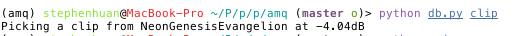
\includegraphics[scale=0.7]{clip.png}
      \caption{Generating a clip from an anime intro.}
    \end{subfigure}
    
    \begin{subfigure}[h]{0.3 \textwidth}
      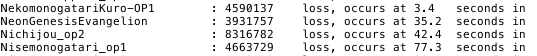
\includegraphics[scale=0.5]{compare.png}
      \caption{Comparison between songs; finds it occurs exactly 35.2 seconds in.}
    \end{subfigure}
    \hfill
    \begin{subfigure}[h]{0.3 \textwidth}
      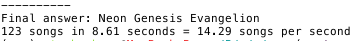
\includegraphics[scale=0.5]{result.png}
      \caption{Song with the lowest loss.}
    \end{subfigure}
    \caption{An example run of the system.}
\end{figure}

First, some basics about the representation of audio data. We will use the
mp3 file format at a sample rate of 48kHz. 
Audio is fundamentally just a list of numbers, where each number represents
the amplitude of the sound wave at that time. A 48kHz sample rate means 
there are 48,000 of these measurements per second.
Each number is a 16-bit number in the range \( [0, 1) \), which we
will transform to an integer in the range \( [0, 2^{16}) \) for the NTT.
So we have two lists of integers, and now wish to find where the smaller list
\enquote{fits} into the larger list the best. One way to do this is to compute
the \emphasis{\( \ell^2 \) norm}, or the vector difference between the two lists.
So we slide the smaller list over the larger list, computing the sum of squares
error as we go. Note that this is very similar to the convolution, except
we to calculate the sum of squares instead of the element-wise product.
We also need to flip one of the lists because the convolution flips a list.

How do we reduce sum of squares to an element-wise product? We notice that
\( (a_i - b_j)^2 = a_i^2 - 2a_i b_j + b_j^2 \) for elements of the lists
\( a, b \). When we sum over the length of \( a \) (assuming \( a \) is the 
smaller list), we get \( \norm{a}^2 - 2 a \cdot b' + \norm{b'}^2 \),
where \( b' \) is the slice that \( a \) overlaps. \( \norm{a} \) is a constant,
so it can be ignored. Thus, we only need to compute \( a \cdot b' \) and
\( \norm{b'} \). \( a \cdot b' \) directly follows from a convolution and
can be read from \( a * b^r \), where \( b^r \) is the reverse of \( b \).
Lastly, if we make sure to scan from left to right, then we can compute
\( \norm{b'} \) by storing an intermediate value, and updating it when we slide 
\( a \) an additional index by subtracting out the front of \( b' \), where
\( a \) left from, and adding the new value that \( a \) covers.

\begin{algorithm}
  \caption{minimum \( \ell^2 \) between two lists}
  \begin{minted}[frame=none]{python}
  def min_offset(a: list, b: list) -> tuple:
      N, M = len(a), len(b)
      p = fft(a[::-1], b)[N - 1:]
      x2, xy, y2 = sum(x*x for x in a), p[0], \
                   sum(b[i]*b[i] for i in range(N))
      best, l2 = 0, -2*xy + y2
      for i in range(1, M - N + 1):
          y2 += b[N - 1 + i]*b[N - 1 + i] - b[i - 1]*b[i - 1]
          xy = p[i]
          d = -2*xy + y2
          if d < l2:
              best, l2 = i, d
      return best, x2 + l2
  \end{minted}
\end{algorithm}

We need to be careful about a few things. If we don't pick \( p \) for the NTT
large enough, then it won't work. If \( m \) is the largest number in a list
and \( n \) is the length of the list, then we need \( p \) to be bigger than
\( m^2 n \) (the largest a single element can become).
\( n \) is \( 90 \cdot 48,000 \approx 4 \cdot 10^6 \) and \( m \) is
\( 2^{16} \). \( m^2 n = 2^{32} \cdot 4 \cdot 10^6 \approx 2^{54} \).
This seems fine since \( 2^{54} \) will fit in a long, but this won't work
since we need to compute \( x^2 \) as part of the FFT, and \( (2^{54})^2 \)
will definitely overflow. We could get around this overflow by doing modulo
multiplication instead of standard multiplication, but that would introduce
a log factor, making the algorithm 64x slower, an unacceptable slowdown.
One trick is to reduce the bitrate of the mp3
at the sacrifice of audio quality, and go from 16-bit audio to 8-bit audio.
A naive way to do it would be to multiply the real number by \( 2^8 \) and
round, but a better way is the \( \mu \)-law algorithm, a trick that preserves
frequencies closer to the human voice. A comparison between naive scaling
and the \( \mu \) law is presented
\href{https://www.youtube.com/watch?v=PqkE_t5cCoA}{here}.
With 8-bit audio, \( m^2 n = 2^{16} \cdot 4 \cdot 10^6 \approx 2^{38} \).
This goes over the limit of \( 2^{32} \) for \( x^2 \) to fit in a long,
but it works in practice since mp3 audio rarely hits maximum volume and
our clip is 10 seconds long, and we computed for 90 seconds.

As mentioned in the NTT, we also need to avoid negative numbers. If we have a
value greater than \( \frac{p}{2} \), we assume it is negative and subtract
\( p \) from it to get its proper value, otherwise we keep the value the same.
\begin{minted}[label=accounting for negative values]{python}
def ntt_sign(l: list, p: int) -> list:
    return [x if x < (p >> 1) else x - p for x in l]
\end{minted}

An implementation is given
\href{https://github.com/stephen-huan/anime-music-quiz}{here} and a video
walkthrough \href{https://www.youtube.com/watch?v=7fUicc_lIGA}{here}.

\newpage

\section{2D Convolutions}
2D convolutions, a convolution generalized to matrices, are useful in computer
vision for a variety of reasons, including edge detection and convolutional
neural networks. Their exact usage will not be discussed here, and instead
we will discuss an efficient way to calculate a 2D convolution with the FFT we 
have already developed. We have an \enquote{data} matrix, representing an image,
and we have a \emphasis{kernel} matrix, which is the matrix we imagine
sliding over the image. This is also known as a \emphasis{filter}.

For 2D convolutions, the result is slightly ambiguous depending on how one
defines it. We will use
\href{https://docs.scipy.org/doc/scipy/reference/generated/scipy.signal.convolve2d.html}{scipy's}
definition, where to calculate the value of the convolution at a particular
point, we imagine the \textit{bottom right} corner of the kernel
placed over that point.

\begin{figure}[h!]
  \centering
  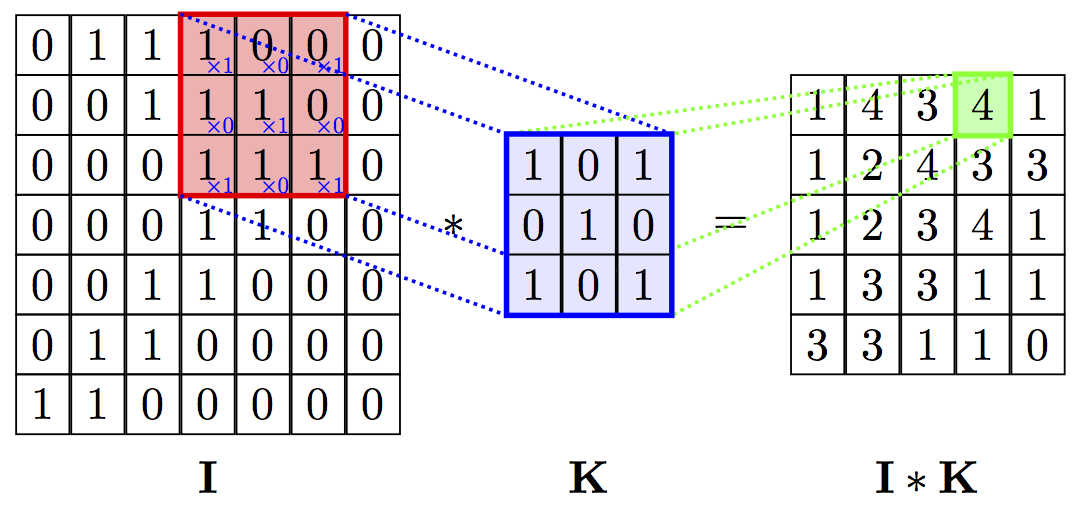
\includegraphics[scale=1.4]{conv.png}
  \caption{A convolution taken from \href{https://petar-v.com/GAT/}{here}.}
\end{figure}

We define the 2D convolution between an image \( x \) of size \( M \)x\( N \)
and a kernel \( h \) of size \( H \)x\( W \) as follows
(similar to the 1D case, we assume both matrices are padded with 0's):
\[ (x * h)[i, j] = \sum^i_{k = 0} \sum^j_{l = 0} x[k][l]h[i - k][j - l] \]

This operation is also symmetric, so  what we call the image and the kernel
is essentially arbitrary (by convention, the kernel is the smaller matrix).
The resulting matrix is going to be of size \( (M + H - 1) \)x\( (N + W - 1) \)
from the same logic as the 1D case. 
Thus, the time it takes to compute the convolution is \( O(MNHW) \).
We can, however, take advantage of a trick if the kernel has a certain property.

\subsection{Separable Kernels}
A matrix \( M \) is \emphasis{separable} if it can be written as
\( \vec{u} \vec{v}^T \) for some vectors \( \vec{u}, \vec{v} \).
For example, the famous Sobel matrix for edge detection is separable:
\[
  \begin{bmatrix}
    1 & 0 & -1 \\
    2 & 0 & -2 \\
    1 & 0 & -1
  \end{bmatrix}
  =
  \begin{bmatrix}
    1 \\
    2 \\ 
    1
  \end{bmatrix}
  \begin{bmatrix}
    1 & 0 & -1
  \end{bmatrix}
\]
If a matrix is separable, we can convolute with
\( \vec{u} \) and then with \( \vec{v} \).

\begin{theorem}
  If \( h = \vec{u} \vec{v}^T \), then \( (x * h) = ((x * \vec{u}) * \vec{v}) \),
  i.e. we can separate a convolution into two parts.
\end{theorem}
\begin{proof}
  \begin{align*}
    (x * u)[i, j] &= \sum^i_{k = 0} \sum^j_{l = 0} x[k][l]u[i - k][j - l] &&
    \text{Definition} \\
    \shortintertext{Since \( u \) is a column vector, it only has values when
    \( l = j \), removing the inner sum.}
                  &= \sum^i_{k = 0} x[k][j]u[i - k][0]
    \shortintertext{Convoluting with \( v \),}
    ((x * u) * v)[i, j] &= \sum^i_{k = 0} \sum^j_{l = 0} (\sum^k_{m = 0} x[m][l]u[k - m][0]) v[i - k][j - l] \\ 
    \shortintertext{Since \( v \) is a row vector, it only has values when
    \( k = i \), removing the outermost sum.}
                        &= \sum^j_{l = 0} (\sum^i_{m = 0} x[m][l]u[i - m][0]) v[0][j - l] \\ 
    \shortintertext{Swapping the order of summations and
    renaming \( m \) to \( k \),}
                        &= \sum^i_{k = 0} \sum^j_{l = 0} x[k][l]u[i - k][0] v[0][j - l] \\
    \shortintertext{From the fact that \(h[x][y] = u[x][0] v[0][y] \),}
                        &= \sum^i_{k = 0} \sum^j_{l = 0} x[k][l]h[i - k][j - l] \\
                        &= (x * h)
  \end{align*}
\end{proof}

How does this help us? Well, recall the running time of \( O(MNHW) \).
If we do two convolutions of a kernel of \( H \)x1  and another of 1x\( W \),
the running time will be \( O(MNH + MNW) = O(MN(H + W)) \), a significant
improvement as \( HW \) grows quadratically while \( H + W \) grows linearly.
We can also use repeated 1D convolution to compute the 2D convolution for the
specific case of a vector, yielding a \( O(MN \log MN) \) time algorithm.

However, not every matrix is separable. The conditions are quite strict,
a matrix is separable if and only if every pair of rows is a multiple of each
other, i.e. the matrix is made up of multiples of a particular row vector.
As a consequence, the matrix is also made up of multiples of a particular
column vector. These matrices are relatively rare, so there is utility
in deriving a more general algorithm.

\subsection{FFT Algorithm}

We can reduce 2D convolutions to 1D convolutions if we're clever.
The observation is that if we \emphasis{flatten} both matrices into a 1D list
by reading from top to bottom, left to right, we can just convolute in 1D
and reconstruct the matrix afterwards. We need to make sure both matrices
are sufficiently padded with zeros, such that the zeros force values
in the kernel to their proper rows in the image. It turns out that we can
just pad both matrices to the final column size of the convolution, 
\( N + W - 1 \), flatten both, convolute with the FFT, and then reshape the
resulting list to a matrix of proper size.
\begin{algorithm}
  \caption{2D Convolution Algorithm}
  \begin{minted}[frame=none]{python}
def flatten(m: list, pad=0) -> list:
    """ Flattens a matrix into a list. """
    return [x for row in m for x in row + [0]*pad]

def reshape(l: list, m: int, n: int) -> list:
    """ Shapes a list into a MxN matrix."""
    return [[l[r*n + c] for c in range(n)] for r in range(m)]

def conv(h: list, x: list):
    """ Computes the 2D convolution. """
    M, N, H, W = len(x), len(x[0]), len(h), len(h[0])
    # need to pad the columns to the final size
    h, x = flatten(h, N - 1), flatten(x, W - 1)
    return reshape(fft(h, x), M + H - 1, N + W - 1)
\end{minted}
\end{algorithm}
In most computer vision applications, the kernel is a square matrix
of size \( K \)x\( K \), where \( K \) is an odd number.
The \textit{middle value} of the kernel is then placed over each pixel of the
image, yielding a transformed image of the same dimensionality as the original.
We can simulate this by simply cutting off the first and last
\( \frac{K - 1}{2} \) rows and the same for the columns.
This transforms the resulting size from \( N + K - 1 \) to
\( N + K - 1 - 2 \frac{K - 1}{2} = N \).

\begin{minted}[label=pruning]{python}
def prune(h: list, x: list) -> list:
    """ Prunes a convolution for the specific KxK filter case. """
    m, k = conv(h, x), min(len(h), len(x))
    pad = (k - 1)>>1
    return [row[pad:-pad] for row in m[pad:-pad]]
\end{minted}

\newpage

The running time of the algorithm is going to be
\( O(MN \log MN) = O(MN(\log N + \log M) = O(MN \log N) \) since we convolute 
a list of length \( M(N + W - 1) \), and we assume \( N \geq M > W \).
This is not necessarily faster than the brute-force algorithm;
it depends on the kernel size. For simplicity, suppose we have a \( N \)x\( N \)
image and a \( K \)x\( K \) kernel where \( N > K \). Brute force yields
\( O(N^2 K^2) \) while the FFT algorithm yields \( O(N^2 \log N) \).
Thus, if \( \log N < K^2 \) then the FFT algorithm is going to be faster.
For \( K > 5 \) that is a fair assumption since \( K^2 = 25 \), \( 2^{25} \)
is several million. Obviously the FFT algorithm has a much larger constant
factor, but for a sufficiently large kernel the time savings become greater
and greater.

\section{Conclusion}

The convolution, an operator very useful for signal, audio, and image
processing, can be efficiently computed with the Fast Fourier Transform, or FFT.
If the data is integer, then floating-point arithmetic can be avoided with the
Number Theoretic Transform (NTT), a variant of the FFT which uses modulo
instead of complex numbers, and calculates entirely in integers.

This lecture skips over the continuous case (what I've been calling the 
Fast Fourier Transform is more mathematically called the
\emphasis{Discrete Fourier Transform}, or DFT) but the idea is essentially the
same, any summation turns into an integral. It also skips over the mathematical
interpretation of the FFT, involving decomposing a function into a series of
sine and cosine waves. This is useful for signal processing and audio analysis,
but requires a stronger mathematical background and to be honest, I haven't
studied it at all myself. Fourier analysis goes deeper than we need here. 

\textit{Introduction to Algorithms} is definitely the most helpful source on
the FFT (from a computer science perspective), and more thorough treatments of
the FFT from an engineering or mathematical standpoint are not hard to find.

\newpage

\section{Sample Problems}

\begin{enumerate}
  \item \href{https://www.spoj.com/problems/POLYMUL/}{SPOJ POLYMUL}:
    Direct application of the FFT.

  \item \href{https://www.spoj.com/problems/MUL/}{SPOJ MUL}:
    Given 1000 pairs of numbers, compute the product of each pair;
    each number can have up to 10,000 digits.

    Solution: Think of numbers as polynomials, where the digits are coefficients
    and \( x \) is 10. Then, you can multiply two numbers by multiplying the
    polynomials. However, there is no guarantee that the coefficients
    of the resulting polynomial are less than 10, so it is not a valid number.
    As a last post-processing step, start from the smallest place value
    and move your way to the largest, moving the digit overflow from one place
    value to the next. Since you iterate over the number of digits in the
    number, it takes \( O(\log n) \) which is dominated by the FFT.
    
    An extension of this idea is the 
    \href{https://en.wikipedia.org/wiki/Sch%C3%B6nhage%E2%80%93Strassen_algorithm}
    {Schönhage–Strassen} algorithm, which disregards the requirement
    that the intermediate numbers fit in a long, at the cost of being
    \( O(n \log n \log \log n) \). A more recent algorithm,
    by Harvey and van der Hoeven, achieves 
    \href{https://hal.archives-ouvertes.fr/hal-02070778/document}{\( O(n \log n) \)}.

  \item \href{https://www.spoj.com/problems/MAXMATCH/}{SPOJ MAXMATCH}:
    Given a string \( S \) of length \( N \) made up of the characters
    \enquote{a}, \enquote{b}, and \enquote{c}, compute the maximum
    self-matching, where a self-matching is defined as the number of characters
    which match between \( S \) and \( S \) shifted some
    nonzero number of characters.

    Solution: For an offset \( i \), the size of the overlap
    will be \( N - i \). So we just need to find the number of differences,
    and subtract that from \( N - i \) to obtain the number of matches.
    The easiest thing to do is to keep track of each character separately,
    so to compute the differences for each character.
    Suppose our character is \enquote{a}. We encode \enquote{a} as a 0,
    and the other characters as a 1. We then find the \( \ell^2 \) norm between 
    this new list and this list with \( N \) 1's added to it
    (so that when we overlap, the non \enquote{a} characters aren't counted).
    This has the complication of counting \enquote{a}'s which are off the edge
    of the string, which we can account for by simply keeping track of the 
    number of \enquote{a}'s we have seen.

    Given \( a[i] \) as the number of mismatches with the character \enquote{a}
    at a shift of \( i \), and \( b[i], c[i] \), the number of matches is 
    \( N - i - \frac{a[i] + b[i] + c[i]}{2} \). We divide by 2 because we
    count each mismatch twice (once for each character in the pair).

    A much conceptually simpler algorithm is to encode \enquote{a}, \enquote{b},
    and \enquote{c} cleverly and then compute the matches in one shot. 
    If we encode \enquote{a} as (1, 0, 0), \enquote{b} as (0, 1, 0), and
    \enquote{c} as (0, 0, 1), the FFT of the resulting list with its reverse
    will give us the number of matches at each index because the character
    representations dot each other will be 1 if they are equal, and 0 
    if they are unequal. Thus, the FFT will give us exactly the number of
    matches, but we need to only look at every 3rd index since the other 2
    are byproducts of our transformation.

    In practice, running one big FFT is faster than running 3 smaller FFTs.

  \item \href{https://www.codechef.com/problems/FARASA}{Codechef FARASA}:
    Given an array, find the number of distinct sums of a contiguous subarray.

    Solution: \href{https://discuss.codechef.com/t/farasa-editorial/2688}
    {editorial}.

    Fair warning, time bounds are ridiculous.

  \item \href{https://codeforces.com/contest/528/problem/D}
    {Codeforces Round \#296}: Given two strings \( T, S \) and 
    an error bound \( k \), find all the positions where \( T \) occurs
    in \( S \), where \( T \) \enquote{occurring} at some index \( i \) 
    means that the \( j \)th character of \( T \) has a corresponding character
    within \( k \) of its position.

    Solution: Honestly no clue but it has the \enquote{FFT} tag.

  \item \href{https://cs.stanford.edu/~rishig/courses/ref/l17.txt}
    {String matching with wildcards}: Given two binary strings \( T, S \),
    \( T \) has length \( N \) and has wildcards which match any character
    in \( S \), find all occurrences of \( T \) in \( S \).

    Solution: Encode 1 as 1 and 0 as -1. The dot product between \( T \)
    and the slice that \( T \) overlaps with \( S \) will be be \( N \)
    if they match exactly and less than \( N \) if they don't match exactly.
    To account for wildcards, encode a wildcard as \( 0 \) and count the
    number of wildcards, \( C \). Then, if they match exactly it will be
    \( N - C \), and less then that if they don't.

    This can be generalized to non-binary strings if you apply the above
    algorithm to each character, setting that character as 1 and not that
    character as -1. Sum over all possible characters, and that will tell you
    whether there is a mismatch somewhere (similar to SPOJ MAXMATCH).

    This idea can also be applied to string matching without wildcards.
    Encode each character as its ASCII value in a polynomial, and compute
    the \( \ell^2 \)-norm between \( T \) and \( S \). The \( \ell^2 \) norm
    will be 0 if they match, and positive if they don't.

  \item \href{https://en.wikipedia.org/wiki/3SUM}{3SUM}:
    Given a list of integers between \( -N \) and \( N \),
    find 3 numbers that add up to 0 (duplicates are allowed). 

    Solution: The basic idea will be to encode the list into a length \( 2N \)
    polynomial \( p \) where the degree is an integer value and the coefficient
    is whether that value appears in the array.
    Compute \( p^3 \) and read off the coefficient of \( x^0 \).
    However, this doesn't work if the degrees are negative. If the most negative
    power of \( x \) in \( p \) is \( x^{-N} \), We can simply multiply \( p \)
    by \( x^N \) to make every power positive, making a new polynomial \( p' \).
    Then, after computing \( (p')^3 \), instead of looking at the coefficient of
    \( x^0 \), we can look at the coefficient of \( x^{3N} \)
    (accounting for the fact that \( p' = x^N p \), \( (p')^3 = x^{3N} p^3 \),
    \( p^3 = \frac{(p')^3}{x^{3N}} \)

    Alternative solution, if duplicates aren't allowed:
    \href{https://cs.stanford.edu/~rishig/courses/ref/l16.txt}{here}
    (look for \enquote{color coding}).

  \item \href{https://animemusicquiz.com/}{Anime Music Quiz}:
    Guess which anime an intro/outro comes from.

    Solution: The \href{https://www.toptal.com/algorithms/shazam-it-music-processing-fingerprinting-and-recognition}
    {Shazam algorithm}.

\end{enumerate}

\newpage

\section{Appendix}
\begin{theorem}
  \( e^{ix} = \cos x + i \sin x \), i.e. Euler's formula 
\end{theorem}
\begin{proof}
  We have the initial value problem (IVP) 
\[ \frac{dy}{dx} = f(x, y), y(x_0) = y_0 \]
\textit{Picard's existence and uniqueness theorem} says that if \( f \) and
\( \frac{\partial f}{\partial y} \) are continuous functions on some rectangle
\( R \) that contains \( (x_0, y_0) \), then the IVP has an unique solution
on some interval \( I \) whose bounds are the regions where the hypotheses hold.

In our particular case, we have \( f(x, y) = iy \) and \( y(0) = 1 \),
so \( \frac{\partial f}{\partial y} = i \). By Picard's theorem, the IVP has a 
unique solution on the interval \( I \) where \( y \) is continuous and
\( \frac{\partial f}{\partial y} \) is continuous. \( i \) is continuous
everywhere, so the IVP will have an unique solution
wherever \( y \) is continuous.

Because this differential equation is separable, we can directly solve
for \( y \).
\begin{align*}
  \frac{dy}{dx} &= iy \\
  \int \frac{1}{iy} dy &= \int dx \\
  \frac{1}{i} \ln{\abs{iy}} &= x + C \\
  \ln{\abs{iy}} &= ix + C \\
  iy &= Ce^{ix} \\
  y &= Ce^{ix} \\
\end{align*}

Taking into account the initial condition, \( y(0) = 1 = Ce^0 = C \).
So \( y = e^{ix} \), which is continuous on \( \mathbb{R} \).
Picard's theorem therefore guarantees the uniqueness of this solution.
However, note that \( \cos x + i \sin x \) is also a solution to the IVP.
First, it fulfills the initial condition since
\( y(0) = \cos 0 + i \sin 0 = 1 \).
Second, it fulfills the differential equation:
\begin{align*}
  \frac{dy}{dx} &= -\sin x + i \cos x \\
                &= i^2 \sin x + i \cos x && \text{Definition of \( i \)} \\
                &= i(\cos x + i \sin x) \\
                &= iy
\end{align*}
Since \( e^{ix} \) is the unique solution to the IVP on \( \mathbb{R} \),
\( e^{ix} = \cos x + i \sin x \).
\end{proof}

\newpage

\section{Past Lectures}
\begin{enumerate}
  \item \href{https://activities.tjhsst.edu/computervision/lectures/Edge_Detection.pdf}
    {\enquote{Edge Detection}}, (Alexey Didenkov, 2018)
  \item \href{https://activities.tjhsst.edu/sct/lectures/1516/SCT_Polynomial.pdf}
    {\enquote{Fast Multiplication: Karatsuba and FFT}} (Haoyuan Sun, 2016)
  \item \href{https://activities.tjhsst.edu/sct/lectures/1415/SCT_Multiplying_Polynomials.pdf}
    {\enquote{Multiplying Polynomials}}, (Haoyuan Sun, 2015)
  \item \href{https://activities.tjhsst.edu/sct/lectures/1213/fft.pdf}
    {\enquote{Fast Fourier Transform}}, (Sreenath Are, 2013)
\end{enumerate}

\section{References}

\begin{enumerate}
  \item \href{https://mitpress.mit.edu/books/introduction-algorithms-third-edition}
    {\textit{Introduction to Algorithms}}, chapter 30 (very helpful)
  \item \href{https://www.nayuki.io/page/number-theoretic-transform-integer-dft}
    {The number theoretic transform}
  \item \href{https://en.wikipedia.org/wiki/%CE%9C-law_algorithm}
    {\( \mu \)-law algorithm}
  \item \href{https://ptolemy.berkeley.edu/projects/embedded/eecsx44/lectures/Spring2013/Picard.pdf}
    {Picard's Existence and Uniqueness Theorem}
  \item \href{https://towardsdatascience.com/a-basic-introduction-to-separable-convolutions-b99ec3102728}
    {Separable convolutions}
\end{enumerate}

% \printbibliography
\end{document}
